\chapter{Face Quality Assessment}
\label{chap:FQA}
The third chapter of the thesis introduces the reader to key definitions and concepts within the field of face quality, used throughout the project. We will throw light on face image quality with examples and elaborate how face recognition systems and the two face image quality metrics behave.  

\section{What Is a Good Image?}
\label{sec:setup}
Throughout this thesis, we will mention the word quality several times. While some people already have a good understanding of what the word means, some confusion may arise. Within the standard image quality assessment field, the definition of quality is straight forward and is what most people think about when hearing the word. Ordinary people and people working with images will for the most part think about an image with a high resolution and no distortion or noise as the most important characteristic that defines image quality. An excellent image of a face with this definition would have a high resolution and a sharp focus. However we are working in the field of biometrics, where the definition differs from this. Our emphasis lies not with the image resolution itself, but with how well the face is visible. There are several aspects that heavily affect the quality of facial images with respect to the performance of biometric systems. These aspects are presented and discussed in two important standards: 
%
\begin{itemize}
    \item ISO/\acrshort{iec} TR 29794-5:2010: Information technology — Biometric sample quality — Part 5: Face image data \cite{ISO50912}.
    \item \acrshort{icao} Doc 9303 Part 3: Specifications Common to all \acrshort{mrtd}s \cite{ICAO1}. 
\end{itemize}

The quality specific aspects of facial images presented in the two standards are what defines the quality in our work. These different quality factors are:  

\begin{itemize}
    \item Scenery characteristics such as lighting or background (Figure \ref{fig:lightning}).
    \item Complete or partial face covering.
    \begin{itemize}
        \item Dark glasses fully covering the eyes (Figure \ref{fig:dark_glasses}).
        \item Any type of face coverings (Figure \ref{fig:face_covering}).
    \end{itemize}
    \item The behaviour of the subject.
    \begin{itemize}
        \item Closed or open eyes (Figure \ref{fig:open_mouth}).
        \item Closed or open mouth (Figure \ref{fig:open_mouth}).
        \item Any kind of expression, e.g., smiling or neutral (Figure \ref{fig:high_quality}).
        \item Head pose, e.g. frontal or rotated in any direction (Figure \ref{fig:side_pose}).
    \end{itemize}
    \item Image properties like the size of the image or its resolution (Figure \ref{fig:poor_resolution}).
    \item Image appearance characteristics like the exposure or noise (Figure \ref{fig:noise}).
    \item Characteristics like the consistency between the skin colour on the image and the skin colour of the subject (Figure \ref{fig:exposure}).
\end{itemize}

The above mentioned aspects all have an affect on the quality of the facial image to some degree. What we consider a high-quality facial image is similar to a standard passport photograph with the following characteristics: 
\begin{itemize}
\label{item:passport}
    \item Open and visible eyes (Figure \ref{fig:lightning}, \ref{fig:face_covering}, \ref{fig:high_quality}, \ref{fig:poor_resolution}, \ref{fig:noise}, \ref{fig:exposure}).
    \item No dark tinted glasses (Figure \ref{fig:lightning}, \ref{fig:face_covering}, \ref{fig:open_mouth}, \ref{fig:high_quality}, \ref{fig:side_pose}, \ref{fig:poor_resolution}, \ref{fig:noise}, \ref{fig:exposure}). 
    \item Neutral or little to none facial expression (Figure \ref{fig:lightning}, \ref{fig:dark_glasses}, \ref{fig:face_covering}, \ref{fig:high_quality}, \ref{fig:noise}, \ref{fig:exposure}).
    \item Neutral face pose (Figure \ref{fig:lightning}, \ref{fig:dark_glasses}, \ref{fig:open_mouth}, \ref{fig:high_quality}, \ref{fig:poor_resolution}, \ref{fig:noise}, \ref{fig:exposure}).
    \item No garments covering the face (Figure \ref{fig:lightning}, \ref{fig:open_mouth}, \ref{fig:high_quality}, \ref{fig:side_pose}, \ref{fig:poor_resolution}, \ref{fig:noise}, \ref{fig:exposure}). 
    \item Clean background (Figure \ref{fig:image_properties}).
    \item Neither too dark or too light background (Figure \ref{fig:dark_glasses}, \ref{fig:face_covering}, \ref{fig:open_mouth}, \ref{fig:side_pose}, \ref{fig:poor_resolution}, \ref{fig:noise}).
    \item Photo taken neither too close or too far away \ref{fig:image_properties}.
\end{itemize} 

Such characteristics will naturally have an affect on the image quality in a good or bad way. If all bullet points above are followed, the quality of the facial image is near perfect. An image of a half-covered or missing face will negatively affect the quality, even though the image resolution itself may be impeccable. 
\begin{figure}[h]
\centering
    \subfloat[A facial image which has the requirements needed for a facial recognition system.]
        {
\includegraphics[width=0.235\textwidth]{figures/0671.jpg}
        \label{fig:excellentImg}\hspace{2.5cm}}\hspace{1.2cm}
    \subfloat[A facial image with defects which does not have the requirements needed for a facial recognition system.]
        {
\includegraphics[width=0.235\textwidth]{figures/0882.jpg}
        \label{fig:defectedImg}\hspace{2.5cm}}
    \caption{Sample images from a face quality dataset.}
\end{figure}
\newpage
Image depicted in Figure \ref{fig:excellentImg} checks all bullet points in what defines a high quality image. The subjects' facial expression and head pose are neutral and the whole face is clearly visible. The second Figure \ref{fig:defectedImg} however, does not have high quality since the face is rotated 90 degrees sideways which only makes half of the face visible. The facial image  in Figure \ref{fig:defectedImg} does have a neutral background with good lightning and image resolution, but those aspects do not weight up against the head pose.
%
\begin{figure}[h]
\centering
    \subfloat[]
        {
\includegraphics[width=.25\textwidth]{figures/0562.jpg} \hfill
        \label{fig:lightning}}
    \subfloat[]
        {
\includegraphics[width=.25\textwidth]{figures/sunglasses.jpg}\hfill
        \label{fig:dark_glasses}}
    \subfloat[]
        {
\includegraphics[width=.25\textwidth]{figures/1078-kopi.jpg}
        \label{fig:face_covering}} \\
        
    \subfloat[]
        {
\includegraphics[width=.25\textwidth]{figures/0867.jpg} \hfill
        \label{fig:open_mouth}}
    \subfloat[]
        {
\includegraphics[width=.25\textwidth]{figures/0457.jpg} \hfill
        \label{fig:high_quality}}
    \subfloat[]
        {
\includegraphics[width=.25\textwidth]{figures/0962-kopi.jpg}
        \label{fig:side_pose} }\\
    
    \subfloat[]
        {
\includegraphics[width=.25\textwidth]{figures/0004photoshop_compression.jpg} \hfill
        \label{fig:poor_resolution}}
    \subfloat[]
        {
\includegraphics[width=.25\textwidth]{figures/0771noise.jpg} \hfill
        \label{fig:noise}}
    \subfloat[]
        {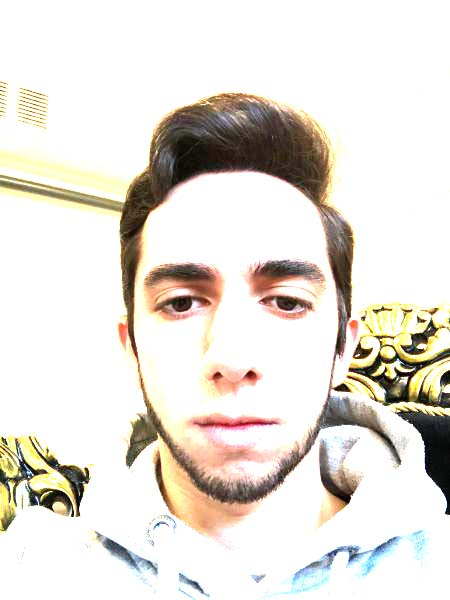
\includegraphics[width=.25\textwidth]{figures/1052exposure.jpg}
        \label{fig:exposure}}
    
\caption{Examples of accepted and not accepted facial images in a facial recognition system.}
\label{fig:image_properties}

\end{figure}

\section{Face Image Quality Metrics} 
With the inclusion of authentication to applications, \acrlong{fr} systems are being utilized more than ever. These FR systems are reliant on a pre-captured reference image (a high quality image) which are then used as a reference to compare with the test image (also called probe image). 

\begin{figure}[h]
    \centering
    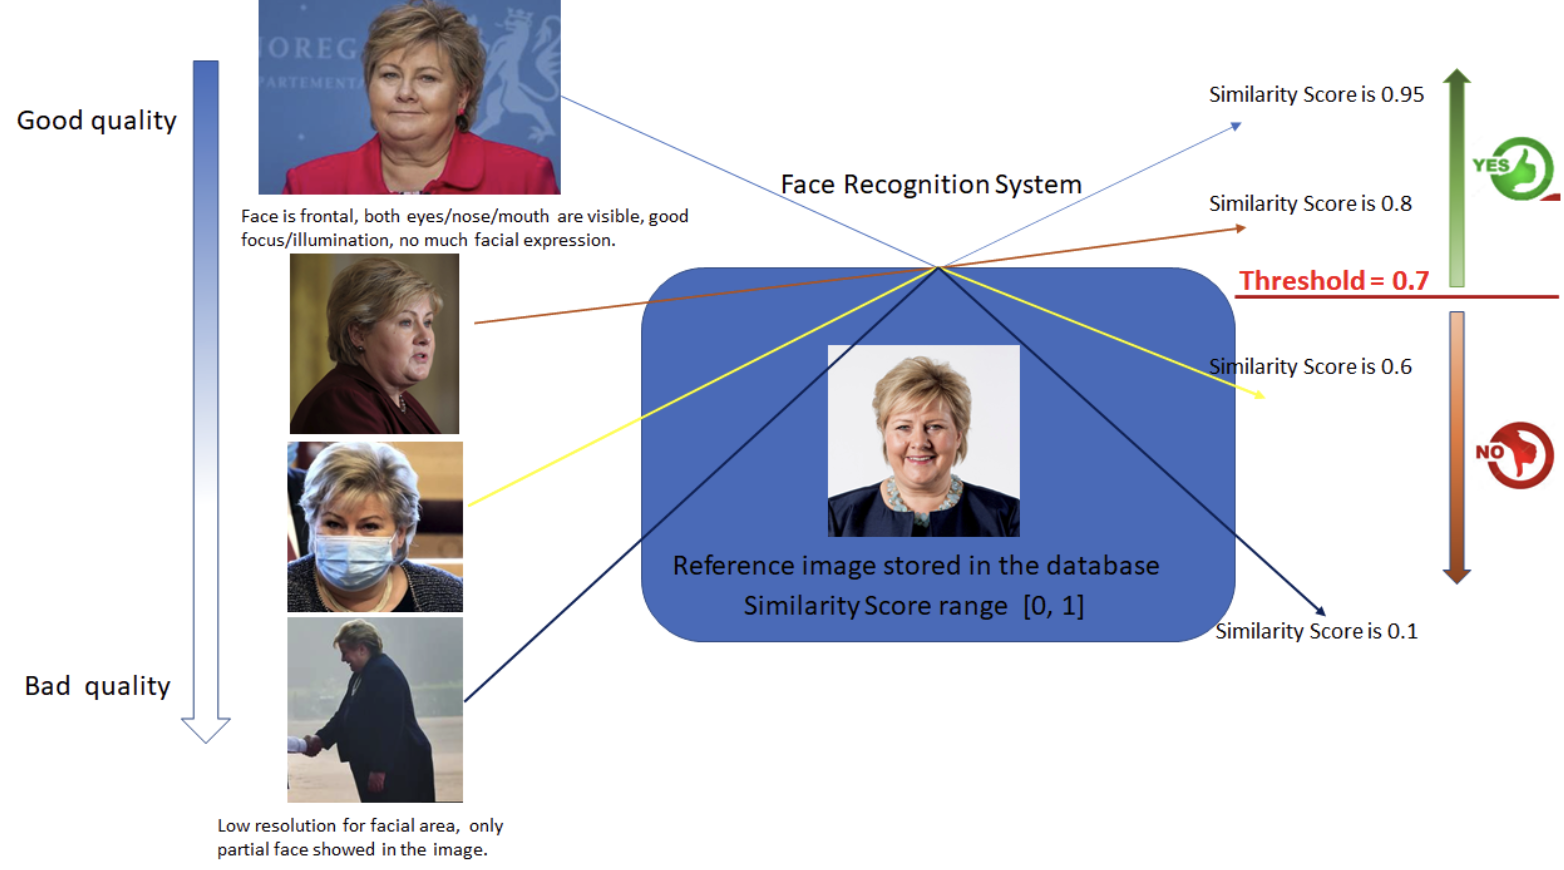
\includegraphics[scale = 0.4]{figures/Erna.png}
    \caption{Face Recognition system. Middle photo by Thomas Haugersveen, Statsministerens Kontor. Top left photo by Human-Etisk Forbund. Second and third from the top photos by Torbjørn Kjosvold, Forsvaret. Bottom left photo by Eirin Larsen, Statsministerens Kontor.}
    \label{fig:erna}
\end{figure}

Figure \ref{fig:erna} visualizes how FR systems work. The quality of the probe images on the left side of the figure are assessed and compared with the reference image. A similarity score between the two images is calculated (in the case of the FR system depicted in Figure \ref{fig:erna} the similarity scores are between zero and one). FR systems have a set threshold where probe images are rejected if the similarity score is too low. 

When it comes to the performance of the system, the quality of the probe images plays a crucial role. If the probe images are of bad quality, the overall performance of the system will decrease. To keep the performance of FR systems, careful attention is paid to the quality of facial images so that only high-quality images are used in the system. For this and to evaluate the quality of facial images, Face Image Quality Metrics (FIQMs) are used.
%
\begin{figure}[h]
    \centering
    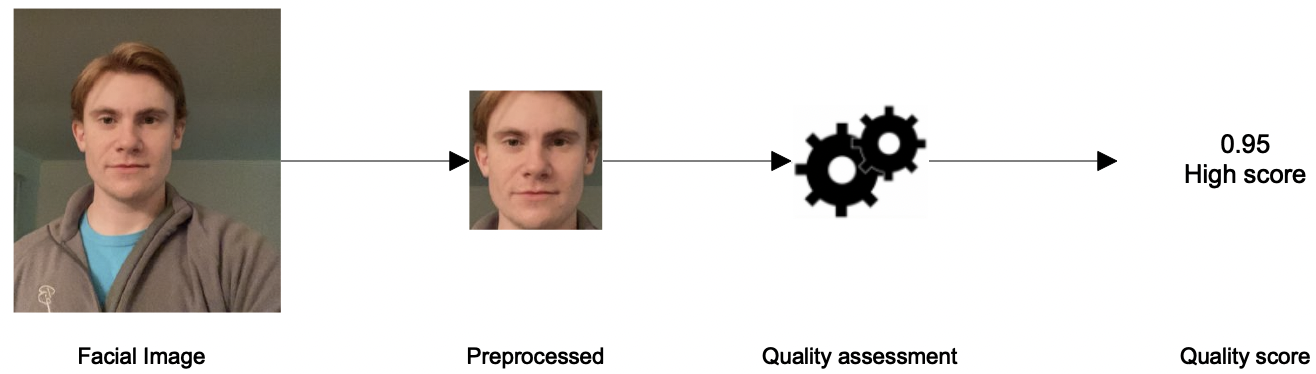
\includegraphics[scale = 0.45]{figures/FIQM_process.png}
    \caption{Typical FIQM process \cite{FaceImageQualityAssessment}.}
    \label{fig:fiqm}
\end{figure}
%
FIQMs are automated algorithms that evaluate the quality of facial images and provide a score which represents the quality of the given images. FIQMs can be based on different quality factors, such as subject-camera distance, inter-eye distance, pose, lightning and facial coverings. % Cite work after each factor

FIQMs can be divided into three approaches in regards to a reference image. It is important to understand that these reference images have nothing to do with the reference images mentioned in the FR systems. These reference images are only used for the FIQMs. The three approaches are: 
%
\begin{itemize}
    \item Full-reference.
    \item Reduced-reference.
    \item No-reference. 
\end{itemize}
%
The names of the approaches are telling of what to expect. The full-reference approach compares the input image with a known reference image of good quality. The reduced-reference approach is similar to the above-mentioned approach, however only some information of the reference image is used. Finally, the no-reference approach does not require a reference image to calculate a score. 

Mobai chose FaceQnet and ISO Metrics to be used in our application. The reason for choosing these specific metrics was their differences in terms of evaluating facial images. The two FIQMs are both no-reference approaches, which will be used to assist and provide feedback when an image is acquired for FR system enrollment. 


\subsection{ISO Metrics}
ISO Metrics is a no-referenced FIQM. The metric is implemented based on ISO/IEC TR 29794-5:2010 Information technology — Biometric sample quality — Part 5: Face image data \cite{ISO50912}. All factors described in the standard affecting the face image quality are implemented in the FIQM. 

The ISO Metrics calculate the inter-eye distance on the facial images. If this value is below a certain score, the metric will filter out these types of images. The inter-eye distance is related to the subject camera distance, because it indicates that the subject could be too close to or to far from the camera lens. 

All image properties and characteristics described in \cite{ISO50912} are taken into account when evaluating the quality of facial images in ISO Metrics. This includes the sharpness, contrast, blur, brightness, exposure, pose symmetry, light symmetry and illumination symmetry of the image. These factors are stored in an array for each facial image. 

To be able to calculate quality scores on the facial images, training data are needed. The metric uses random forest regression \cite{RandomForestRegressor} with 214 estimators and 22 nodes of depth. The quality score for each facial image is computed by predicting the output score of the image properties array.  

\subsection{FaceQnet}
FaceQnet \cite{FaceQnet} is an open source, no-reference FIQM using \acrlong{cnn}s (\acrshort{cnn}s). FaceQnet has two versions implemented, FaceQnet v0 \cite{hernandezortega2019faceqnet} and FaceQnet v1 \cite{hernandezortega2021biometric}. In this project, we used the latest version (FaceQnet v1). Its quality measures are closely related to the ICAO standard \cite{ICAO2} that provides strict guidelines for capturing images. Factors such as illumination, pose, resolution and focus are essential in regard to the final quality score.

A key part of the implementation of FaceQnet is data preprocessing (shown in Figure \ref{fig:fiqm}). Generally data preprocessing removes unnecessary data, which directly improves the quality of machine learning algorithms. The background of images will affect the quality score which provides us with biased results. One way to avoid feature extraction from the background is to crop the input images to only include the face before using FIQMs. FaceQnet uses \acrfull{mtcnn} to detect and extract the coordinates of the face. In the next step, the facial image is cropped to an image with the size $224 \times $224 and used as the input image in FaceQnet v1. 

FaceQnet uses a subset of the VGGFace2 \cite{VGGFace2} dataset to create a pre-trained model to make its quality predictions. The subset consists of 300 subjects. The FIQM will first generate ground truth quality measures which is created by labeling the 300 subjects in the training dataset. The ground truth quality measures will then train the deep regression model in order to generate quality scores. 

